\section{Introducción}

Aquí algunos ejemplos de como se usan las imágenes, las tablas las listas

\textbf{ text in bold}
\textit{text in italics}
\underline{underlined text}
\texttt{text in consola-like font}

\subsection*{Ejemplos de listas}
itemize, enumerate, description

\begin{itemize}
    \item cada item es una viñeta
    \item Otra viñeta
\end{itemize}

\begin{enumerate}
    \item enumeración
    \begin{enumerate}
        \item anidado
    \end{enumerate}
\end{enumerate}

\begin{figure*}[htb]
\centering
\subfloat[] {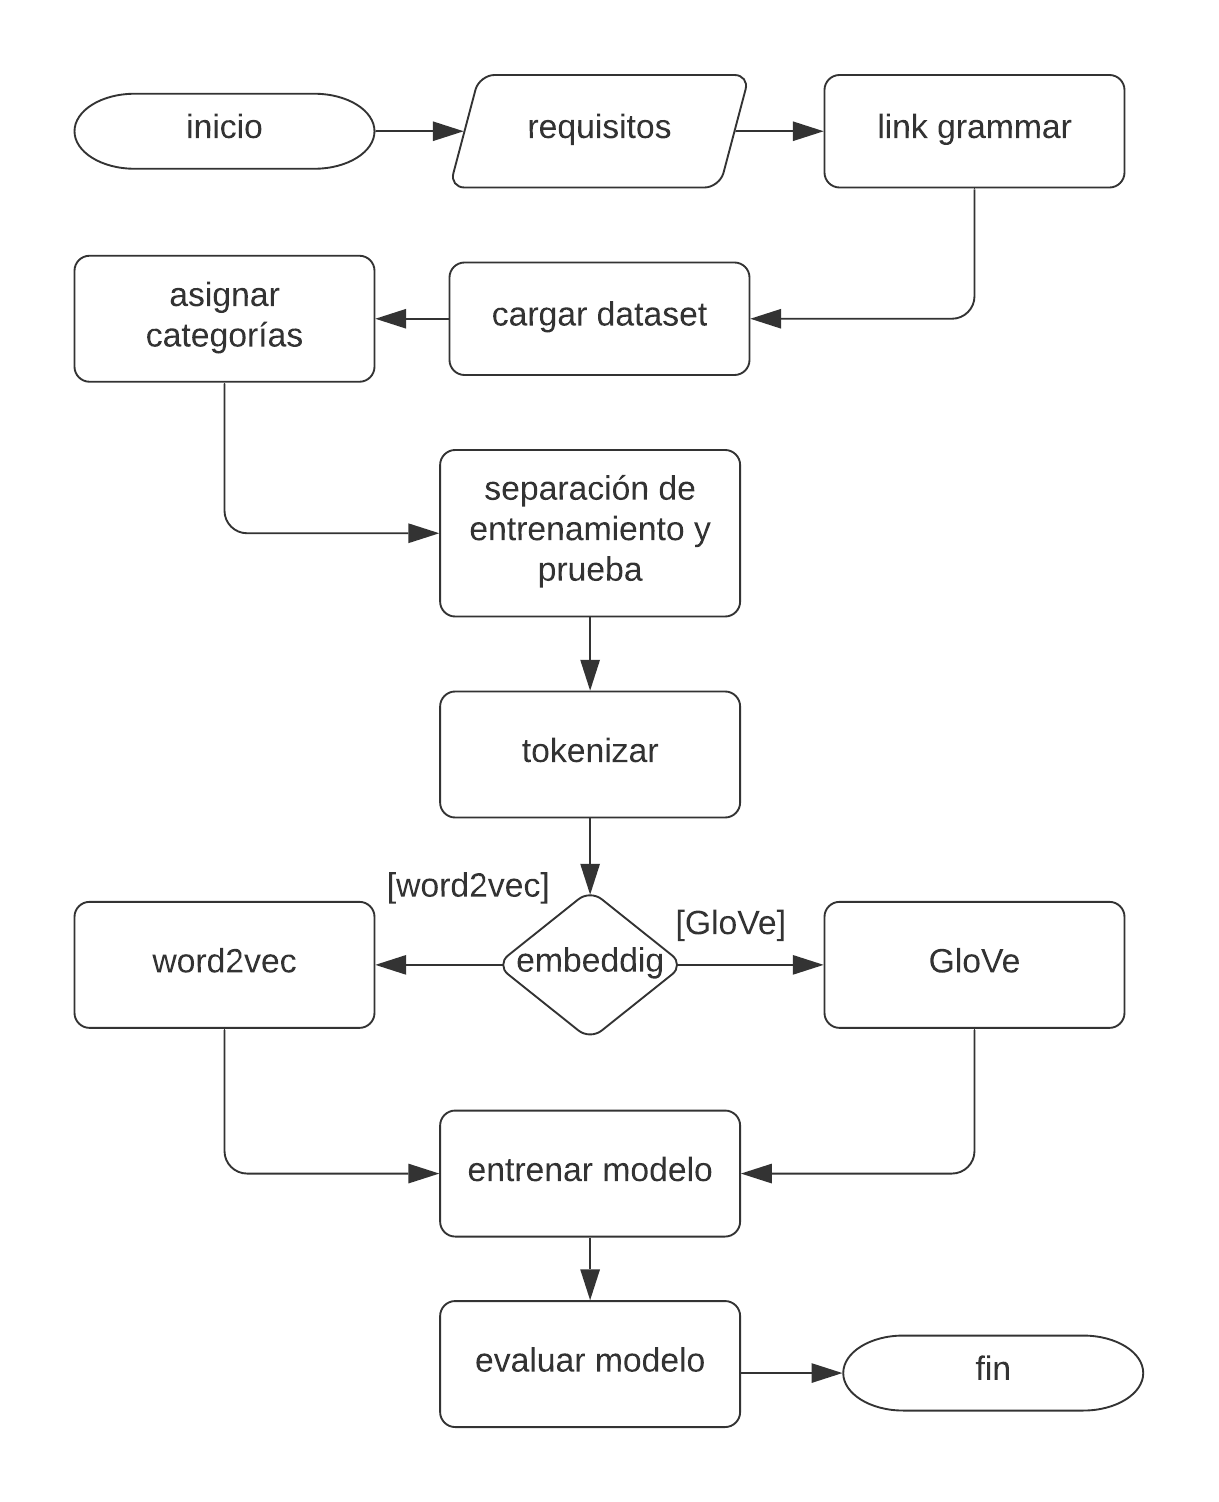
\includegraphics[width=0.5\textwidth]{Deep.png}

\label{fig:PAS_FM}}
\subfloat []{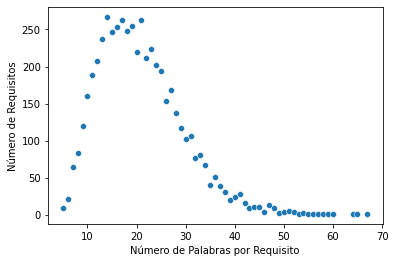
\includegraphics[width=0.38\textwidth]{freq_req.png}

\label{fig:PAS_FM2}}

\label{fig:examples}
\end{figure*}
 
 \begin{table}[htb]
     \centering
     \begin{tabular}{rc}
	\toprule
    	Item1 & Item2  \\
	\midrule
	celda 1 & celda 2\\
	\bottomrule

\end{tabular}
     \caption{Propuesta de elementos identificados en el desarrollo del proyecto. Fuente \citep{Hinton2012}}
     \label{tab:my_label}
 \end{table}

\subsection*{Uso de figuras}
La Figura \ref{fig:figure1} muestra un gráfico de ejemplo. Las tablas y figuras que aparecen en el documento deben ser previamente introducidas y explicadas


\begin{figure}
\centering
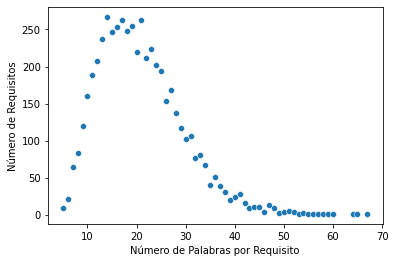
\includegraphics[width=0.5\textwidth]{freq_req.png}
\caption{Grafico tridimensional. Elaboración propia}
\label{fig:figure1}
\end{figure}